\documentclass[dvipsnames,aspectratio=169,pdftex]{beamer}
\usepackage{agda}
\usepackage{stmaryrd}
\usepackage{xcolor}
\usepackage{txfonts}
\usepackage{listings}

\usetheme{Madrid}

\title{Intrinsically Typed Sessions with Callbacks}
\subtitle{Functional Pearl}

\author[Thiemann]
{
\textbf{Peter Thiemann} 
}
\institute{University of Freiburg, Germany
}
\date{September 7, 2023 (ICFP, Seattle, WA, USA)}


\AtBeginSection[]{%
  \begin{frame}<beamer>
    \frametitle{Outline}
    \tableofcontents[currentsection]%[sectionstyle=show/show,subsectionstyle=hide/show/hide]
  \end{frame}
  \addtocounter{framenumber}{-1}% If you don't want them to affect the slide number
}

\usepackage{dsfont}
\usepackage{newunicodechar}
\newunicodechar{λ}{\ensuremath{\mathnormal\lambda}}
\newunicodechar{σ}{\ensuremath{\mathnormal\sigma}}
\newunicodechar{τ}{\ensuremath{\mathnormal\tau}}
\newunicodechar{π}{\ensuremath{\mathnormal\pi}}
\newunicodechar{ℕ}{\ensuremath{\mathbb{N}}}
\newunicodechar{∷}{\ensuremath{::}}
\newunicodechar{≡}{\ensuremath{\equiv}}
\newunicodechar{∀}{\ensuremath{\forall}}
\newunicodechar{ᴸ}{\ensuremath{^L}}
\newunicodechar{ᴿ}{\ensuremath{^R}}
\newunicodechar{ʳ}{\ensuremath{^r}}
\newunicodechar{ⱽ}{\ensuremath{^V}}
\newunicodechar{⟧}{\ensuremath{\rrbracket}}
\newunicodechar{⟦}{\ensuremath{\llbracket}}
\newunicodechar{⊤}{\ensuremath{\top}}
\newunicodechar{⊥}{\ensuremath{\bot}}
\newunicodechar{₁}{\ensuremath{_1}}
\newunicodechar{₂}{\ensuremath{_2}}
\newunicodechar{∈}{\ensuremath{\in}}
\newunicodechar{₀}{\ensuremath{_0}}
\newunicodechar{′}{\ensuremath{'}}
\newunicodechar{ˢ}{\ensuremath{^S}}
\newunicodechar{ᴬ}{\ensuremath{^A}}
\newunicodechar{∘}{\ensuremath{\circ}}
\newunicodechar{𝟙}{\ensuremath{\mathds{1}}}  
\newunicodechar{𝟘}{\ensuremath{\mathds{O}}}
% \newunicodechar{𝟙}{\ensuremath{\mathbb{I}}}  
% \newunicodechar{𝟘}{\ensuremath{\mathbb{O}}}
\newunicodechar{ᴾ}{\ensuremath{^P}}
\newunicodechar{ᵀ}{\ensuremath{^T}}
\newunicodechar{⊎}{\ensuremath{\uplus}}
\newunicodechar{ι}{\ensuremath{\iota}}
\newunicodechar{⇐}{\ensuremath{\Leftarrow}}
\newunicodechar{⇒}{\ensuremath{\Rightarrow}}
\newunicodechar{∎}{\ensuremath{\mathnormal\blacksquare}}
\newunicodechar{➙}{\ensuremath{\to^P}}
\newunicodechar{Δ}{\ensuremath{\Delta}}
\newunicodechar{∅}{\ensuremath{\emptyset}}
\newunicodechar{⁺}{\ensuremath{^+}}
\newunicodechar{𝕏}{\ensuremath{\mathbb{X}}}
\newunicodechar{∙}{\ensuremath{\cdot}}
\newunicodechar{⁇}{\ensuremath{?}}
\newunicodechar{‼}{\ensuremath{!}}
\newunicodechar{⊕}{\ensuremath{\oplus}}
\newunicodechar{ℤ}{\ensuremath{\mathbb{Z}}}
\newunicodechar{μ}{\ensuremath{\mu}}
\newunicodechar{∃}{\ensuremath{\exists}}
\newunicodechar{⨟}{\ensuremath{\fatsemi}}
\newunicodechar{Σ}{\ensuremath{\Sigma}}
\newunicodechar{ᵣ}{\ensuremath{_r}}

\newcommand\Asuc{\AgdaInductiveConstructor{suc}}
\newcommand\Azero{\AgdaInductiveConstructor{zero}}
\newcommand\Anat{\AgdaInductiveConstructor{nat}}
\newcommand\Aint{\AgdaInductiveConstructor{int}}
\newcommand\Abool{\AgdaInductiveConstructor{bool}}
\newcommand\Atend{\AgdaInductiveConstructor{end}}
\newcommand\Atsend[2]{\AgdaInductiveConstructor{‼{\textcolor{black}{\ensuremath{#1}}}∙{\textcolor{black}{\ensuremath{#2}}}}}
\newcommand\Atrecv[2]{\AgdaInductiveConstructor{⁇{\textcolor{black}{\ensuremath{#1}}}∙{\textcolor{black}{\ensuremath{#2}}}}}
\newcommand\ACEND{\AgdaInductiveConstructor{END}}
\newcommand\ACSEND{\AgdaInductiveConstructor{SEND}}
\newcommand\ACRECV{\AgdaInductiveConstructor{RECV}}
\newcommand\ACSELECT{\AgdaInductiveConstructor{SELECT}}
\newcommand\ACCHOICE{\AgdaInductiveConstructor{CHOICE}}
\newcommand\AFin{\AgdaDatatype{Fin}}
\newcommand\ACommand{\AgdaDatatype{Command}}
\newcommand\ACommandStore{\AgdaDatatype{CommandStore}}
\newcommand\ASession{\AgdaDatatype{Session}}
\newcommand\Abinaryp{\AgdaFunction{binaryp}}
\newcommand\Aunaryp{\AgdaFunction{unaryp}}
\newcommand\Aexecutor{\AgdaFunction{exec}}
\newcommand\Aexec{\AgdaFunction{exec}}
\newcommand\AIO{\AgdaFunction{IO}}
\newcommand\Amu{\AgdaInductiveConstructor{\ensuremath{\mu}}}
\newcommand\AMU{\AgdaInductiveConstructor{LOOP}}
\newcommand\ACONTINUE{\AgdaInductiveConstructor{CONTINUE}}
\newcommand\Aback{\AgdaInductiveConstructor{\ensuremath{`}}}
\newcommand\Amanyunaryp{\AgdaFunction{many-unaryp}}
\newcommand\Arestart{\AgdaFunction{restart}}

%%% Local Variables:
%%% mode: latex
%%% TeX-master: "main-icfp23-pearl"
%%% End:


\input{latex/Types.tex}
\input{latex/ST-finite-nonbranching.tex}
\input{latex/Channels.tex}
\input{latex/ST-recursive.tex}
\input{latex/ST-monadic.tex}
\input{latex/ST-indexed-contextfree.tex}
\input{latex/ST-multichannel-finite-branching.tex}
\input{latex/EX-multichannel}
\input{latex/Presentation}

\begin{document}
\begin{frame}{\null}
  \titlepage 
\end{frame}
\begin{frame}
  \frametitle{Session Types}
  \begin{itemize}
  \item Type discipline for communication channels
  \item Prescribes the sequence and direction of messages
  \begin{align*}
    \AT &::= \Aint \mid \Abool  & \AS &::= \Atsend{\AT}{\AS} \mid \Atrecv{\AT}{\AS} \mid \Atend
  \end{align*}
\item Examples
  \end{itemize}
  \PresBinaryUnaryType
\end{frame}
\begin{frame}[fragile]
  \frametitle{Programming with Session Types}
\begin{lstlisting}
negp-server : ?int.!int.end -o ()
negp-server  c0 =                    -- c0 : ?int.!int.end
  let (x, c1) = recv c0 in           -- c1 :      !int.end
  let c2 = send (c1, -x) in          -- c2 :           end
  close c2
\end{lstlisting}
\begin{itemize}
\item Session types are linear
\item Session API transforms the type of channel ends
\end{itemize}
  \begin{align*}
    \mathtt{send} & : \Atsend{\AT}{\AS} \otimes \AT \multimap \AS
    & \mathtt{recv} &: \Atrecv{\AT}{\AS} \multimap (\AT \otimes \AS)
    & \mathtt{close} &: \Atend \multimap ()
  \end{align*}
\end{frame}
\begin{frame}
  \frametitle{This Paper}
  \begin{itemize}[<+->]
  \item A safe session type API without linear types.
  \item A modicum of indexed types / GADTs is sufficient.
  \item Secret sauce: callbacks / first-class functions stored in a
    data structure.
  \end{itemize}
\end{frame}
\begin{frame}
  \frametitle{Origin: Session Types for Web Programming}
  \begin{center}
    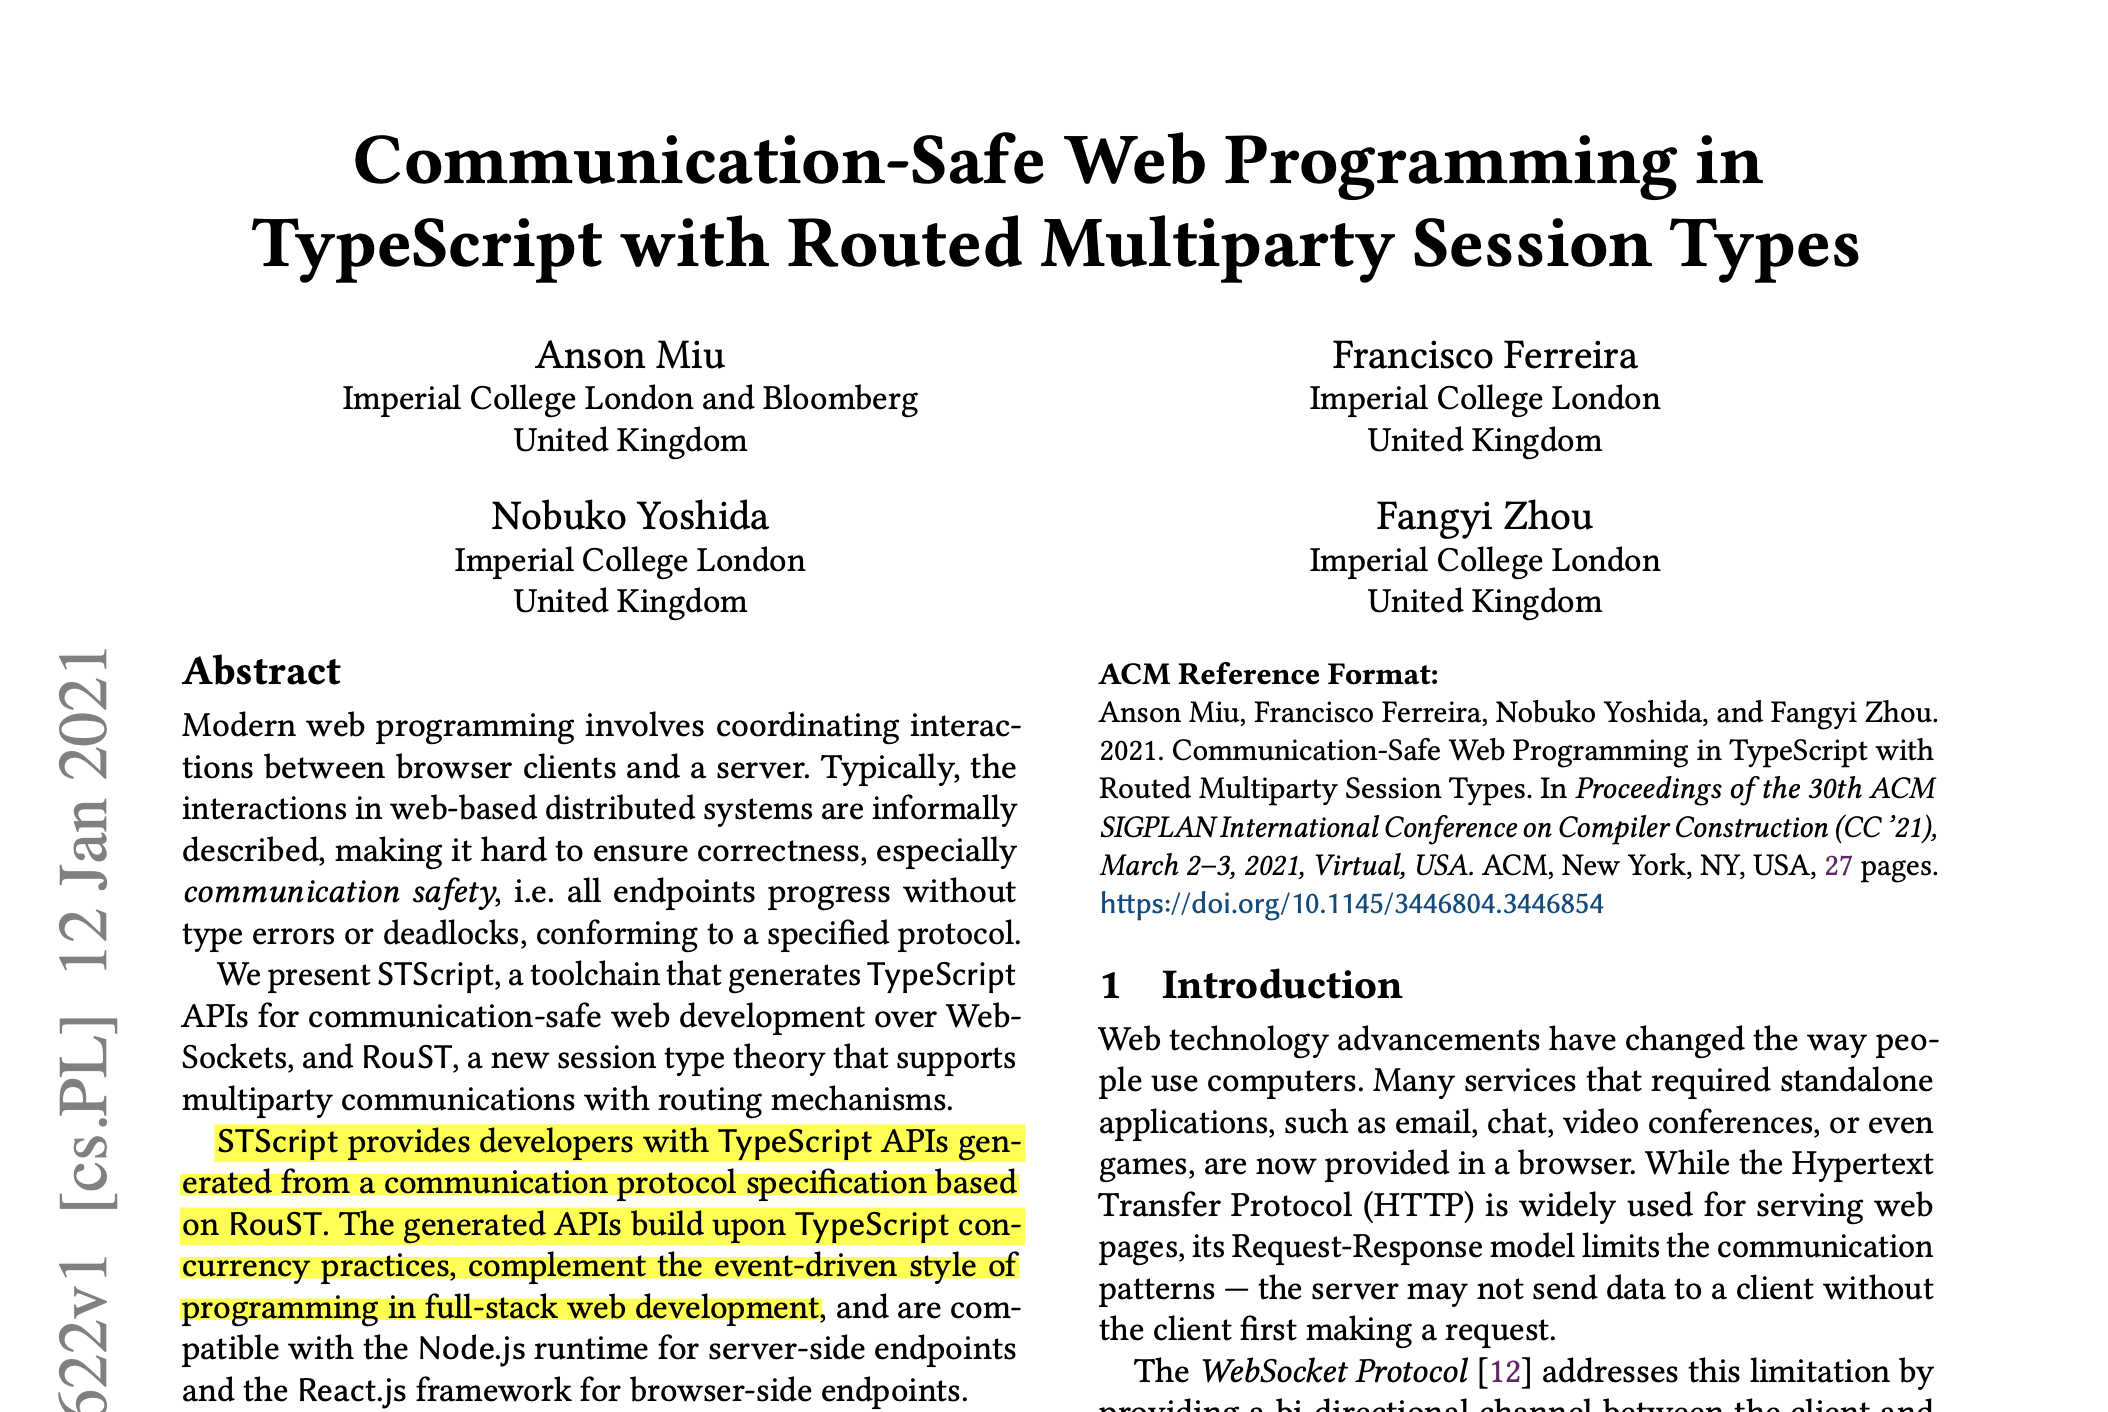
\includegraphics[scale=0.3]{images/routed-titlepage}
  \end{center}
\end{frame}
\begin{frame}
  \frametitle{Origin: Session Types for Web Programming}
  \begin{columns}
    \begin{column}{0.49\textwidth}
      \begin{center}
        \includegraphics<+->[scale=0.45]{images/routed-callback2}
      \end{center}
    \end{column}
    \begin{column}{0.49\textwidth}
      \includegraphics<+->[scale=0.45]{images/handler-interface}
    \end{column}
  \end{columns}
\end{frame}
\begin{frame}
  \frametitle{Callback-Style for Functional Programmers}
  \begin{itemize}[<+->]
  \item No code generation required
  \item No funny generated names in interfaces
  \item Instead: data structure {\ACommand} with embedded callbacks
  \item Using Agda as implementation language
% \item In monadic style:
%   \PresUnaryMonadic
  \end{itemize}
    \begin{columns}<+->
      \begin{column}{0.49\linewidth}
      \PresNegpCommand 
    \end{column}
    \begin{column}{0.49\linewidth}
      \begin{center}
        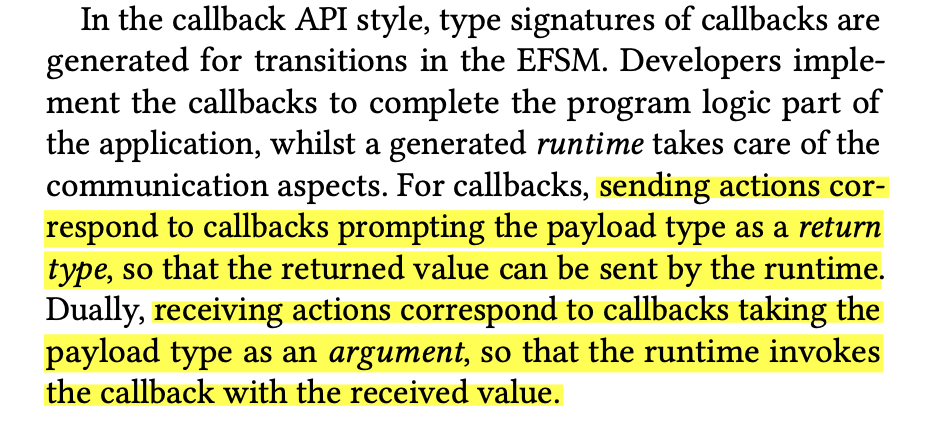
\includegraphics[scale=0.45]{images/routed-send-receive}
      \end{center}
    \end{column}
    \end{columns}
\end{frame}
\begin{frame}
  \frametitle{Encoding of Session Types}
  \begin{columns}
    \begin{column}{0.49\linewidth}
      \stFiniteType
    \end{column}
    \begin{column}{0.49\linewidth}
      \begin{align*}
        \AT &::= \Aint \mid \Abool
      \end{align*}
    \end{column}
  \end{columns}
  \begin{columns}
    \begin{column}{0.49\linewidth}
      \stFiniteSession 
    \end{column}
    \begin{column}{0.49\linewidth}
      \begin{align*}
        \AS &::= \Atsend{\AT}{\AS} \mid \Atrecv{\AT}{\AS} \mid \Atend
      \end{align*}
    \end{column}
  \end{columns}
\end{frame}
\begin{frame}
  \frametitle{Commands}
  \begin{itemize}
  \item Commands working on application state $A$ 
    \stCommand
  \item ``sending actions correspond to callbacks prompting the
    payload type as the return type''
  \item ``receiving actions correspond to callbacks taking the payload
    type as an argument''
  \item Payload types and their interpretation
    \stTypeInterpretation
  \end{itemize}
\end{frame}
\begin{frame}
  \frametitle{Interpretation}
  \begin{columns}
    \begin{column}<+->{0.49\textwidth}
      \stExecutorSignature\vspace{-2\baselineskip} \stExecutor
    \end{column}
    \begin{column}<+->{0.49\textwidth}
      \begin{itemize}
      \item Only place in the system which could break the correct,
        linear handling of the channel
      \item A proof obligation
      \item Currently by inspection, but more could be done
      \end{itemize}
    \end{column}
  \end{columns}
\end{frame}
\begin{frame}
  \frametitle{Selection and Choice}
  \framesubtitle{Modeling}
  \begin{align*}
    \AS  ::= \dots 
      & \mid \oplus\{ \ell : \AS_\ell \mid \ell \in L \}
      && \text{internal choice} \\
      & \mid
        \&\{\ell: \AS_\ell \mid \ell \in L\}
      && \text{external choice}
  \end{align*}
  \begin{itemize}
  \item $L$ a finite set of labels
  \item encoded as $\AFin~k = \{0, \dots, k-1\}$
  \end{itemize}
  \stBranchingType
  \stBranchingCommand
\end{frame}
\begin{frame}
  \frametitle{Selection and Choice}
  \framesubtitle{Example}
  \stExampleBinpUnP
  \stExampleArithP
  \stArithpCommand

\end{frame}
\begin{frame}
  \frametitle{Recursion}
  \framesubtitle{Modeling session types}
  \begin{align*}
    \AS &::= \Atsend{\AT}{\AS} \mid \Atrecv{\AT}{\AS} \mid \Atend \mid
          \underline{\Amu~X. \AS \mid X}
          \mid \dots
  \end{align*}
  \begin{itemize}[<+->]
  \item Modeling variables with de Bruijn indices
    \PresRecSession
  \item Example: $\mu X. \&\{ 0: \Atrecv{\Aint}{\Atsend{\Aint}{X}}, 1: \Atend \}$
    \rstExampleManyUnaryp
\end{itemize}
\end{frame}
\begin{frame}
  \frametitle{Recursion}
  \framesubtitle{Modeling commands}
  \begin{itemize}[<+->]
  \item Commands
    \rstCommand
  \item Issue: {\AMU} handles all loop iterations in the same way
  \item Appropriate for a server, but not for a client
  \item Additional client command $\AUNROLL\ c_1 c_{loop}$ 
    \rstCommandUNROLL
  \item $c_1$ deals with the first iteration, $c_{loop}$ with the
    remaining ones
  % \item Example
  %   \rstSumupCommand
  \end{itemize}
\end{frame}
\begin{frame}
  \frametitle{Recursion}
  \framesubtitle{Interpretation}
  \begin{itemize}
  \item The interpreter maintains a stack of continuations, i.e.,
    pending {\AMU} commands.
    \rstCommandStack
  \item The interpreter only runs to the first {\ACONTINUE} to avoid
    issues with termination.
    \rstCmdCont
  \end{itemize}
\end{frame}
\begin{frame}
  \frametitle{Further Variations in Paper}
  \begin{itemize}
  \item Context-free session types [Thiemann, Vasconcelos, ICFP 2016]
  \item Multichannel session types (runnable)
  \item Monadic callbacks
    % \PresUnaryMonadic
  \end{itemize}
\end{frame}
% \begin{frame}
%   \frametitle{Related Work}
% \end{frame}
\begin{frame}
  \frametitle{Conclusion}
  \begin{columns}
    \begin{column}{0.59\textwidth}
      \begin{itemize}
      \item \textbf{Callback-style} to safely embed session types in a
        language without linear types
      \item \textbf{Indexed types} avoid code generation
      \item \textbf{Many styles of session types} can be encoded
      \item \textbf{Modular protocols and implementations}
      \item Future work: Proof obligations, improve monadic
      \item Check out the artifact, read the paper
      \end{itemize}
    \end{column}
    \begin{column}{0.39\textwidth}
      \begin{center}
        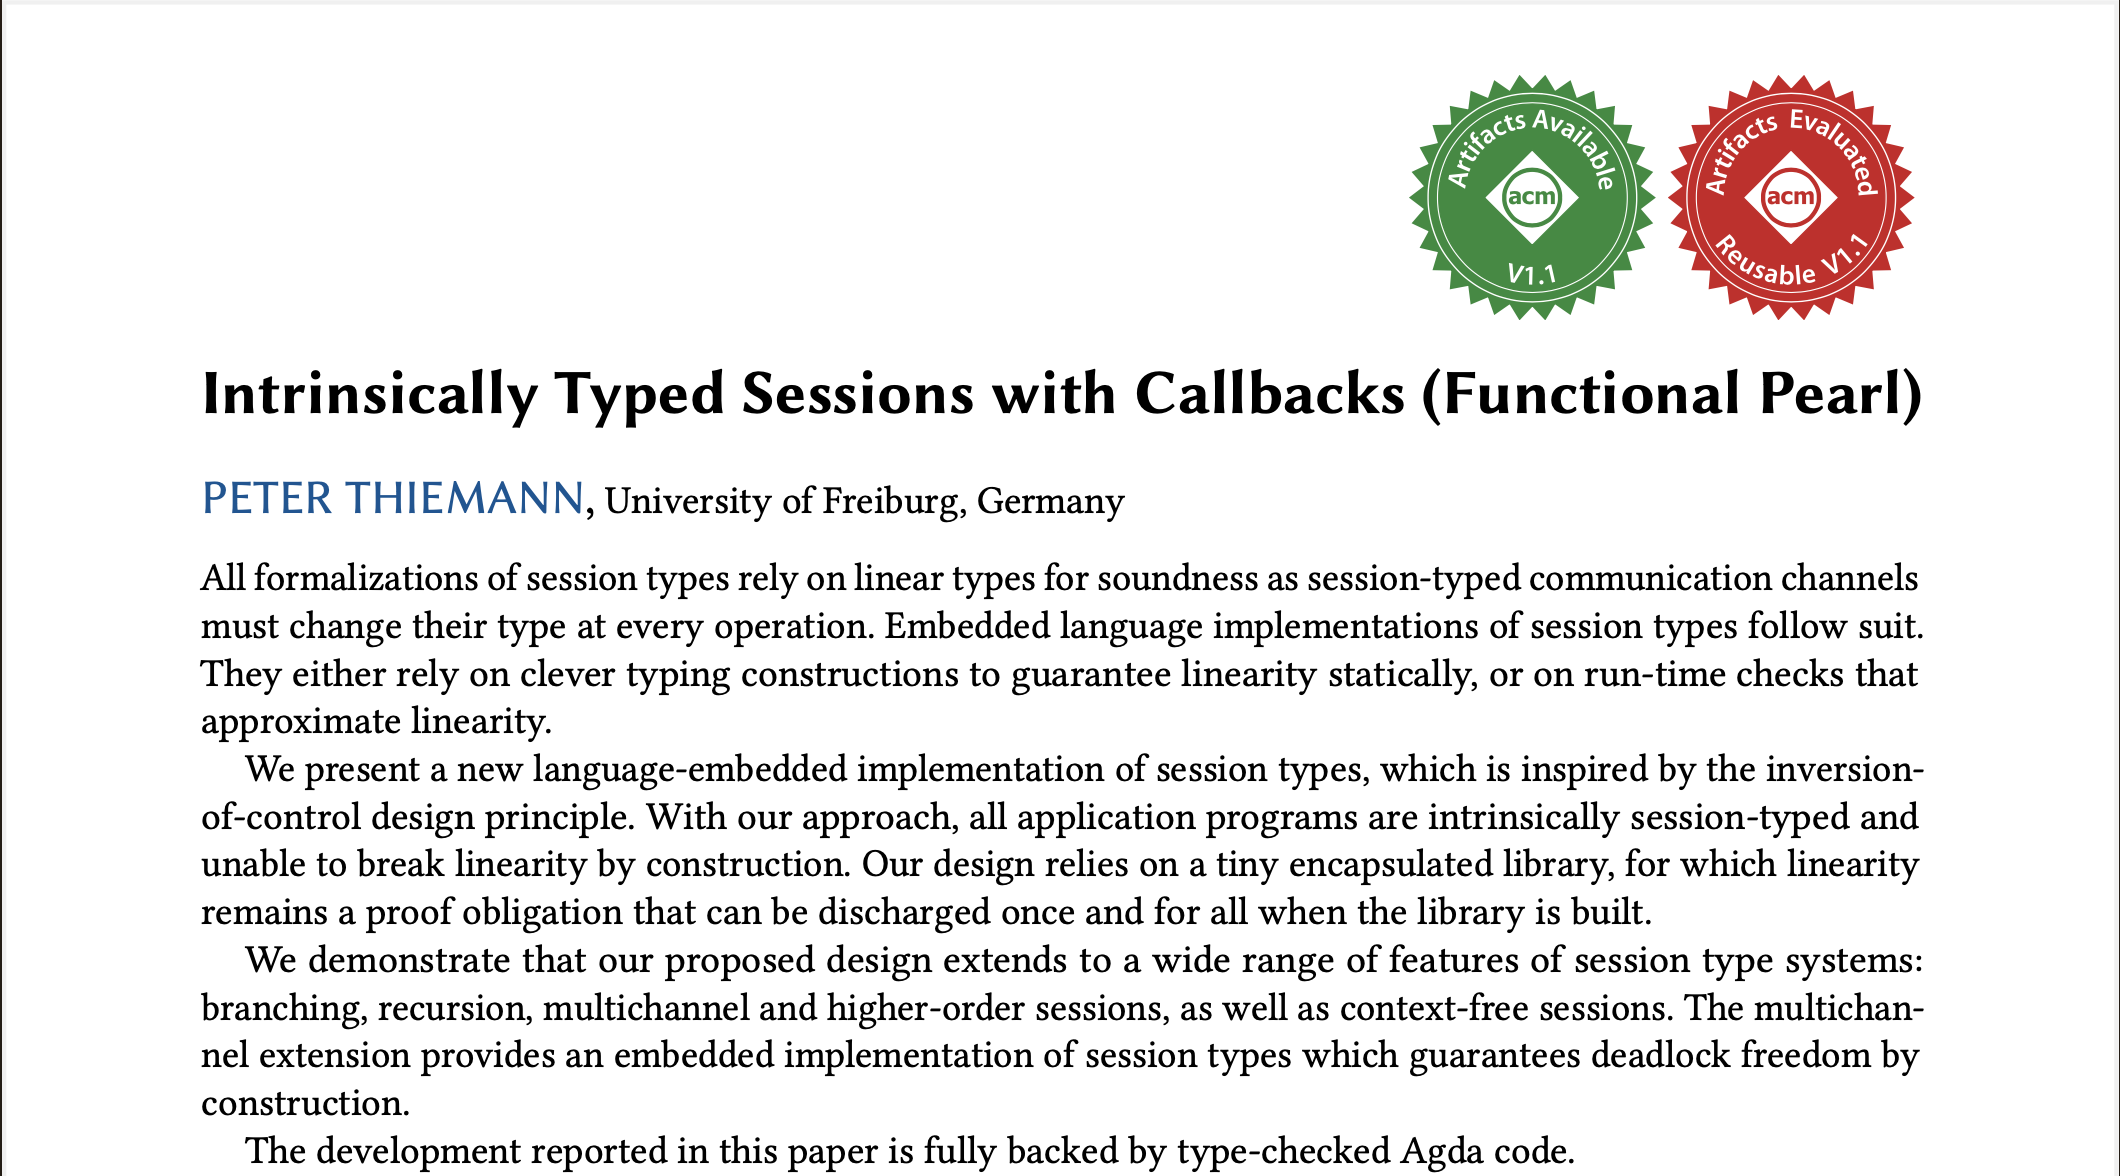
\includegraphics[scale=0.15,trim={0 0 0 0},clip]{images/this-paper}
      \end{center}
    \end{column}
  \end{columns}
\end{frame}
\end{document}
